\chapter{Arquitetura do \textit{framework} de simulação}

Uma vez definida a arquitetura de \textit{middleware} de comunicação a ser utilizado durante este projeto, o próximo passo é a definição do funcionamento e da arquitetura da camada de simulação, aqui genericamente denominado \textit{framework}.

Esta camada, conforme ilustrada na figura~\ref{fig:camada_central}, compreende diversos sub-componentes do framework (aqui esses sub-componentes serão denominados genericamentes de blocos, para que se distingua dos componentes, objetos utilizados para descrever um modelo a ser simulado). Cada bloco que compreende o kernel se liga ao bloco central, denominado \textit{kernel}. Este é o responsável por coordenar a simulação, aplicando sincronização e balanceamento de carga, além de gerenciar o ciclo de vida da simulação (quando começar, quando terminar, etc).

\begin{figure}
  \centerline{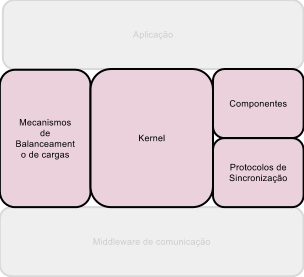
\includegraphics{camada_framework.png}}
  \caption{A camada aqui denominada \textit{framework}.}
\label{fig:camada_central}
\end{figure}

\section{O bloco Componente}

Um componente é uma abstração de um comportamento que desejamos reproduzir na nossa simulação. Na abstração de um sistema de caixa de supermercados, por exemplos, pode-se extrair três componentes (que são comuns em muitas situações na simulação de eventos discretos): o produtor, a fila de espera e o consumidor.

Uma biblioteca de componentes deve proporcionar objetos parametrizáveis que permitam a descrição do comportamento de cada um deles. No caso citado anteriormente, o componete produtor deve suportar parâmetros que, por exemplo, descreva a taxa de criação de novos evento, e as características de cada evento criado.

Os componentes são construidos diretamente em cima do objeto \textit{process} da camada de comunicação. Isso garante ao componente criado, por herança direta, toda funcionalidade de comunicação entre outros componentes. Desta maneira, basta ao usuário do framework descrever na modelagem qual a conexão que cada componente faz, que esta é reproduzida automaticamente pelo framework, independente se esses componentes são processo cohabitantes ou não-cohabitantes.

Em alguns casos é conveniente que componentes sejam combinados a fim de que um novo componente seja criado. Uma das justificativas seria, por exemplo, garantir que doi componentes primitivos se comportem como um único compoente, evitando assim que estes sejam por ventura separados e passem a cohabitar ambientes diferentes. Em um exemplo, é conveniente que o um componente do tipo fila, que tem como características armazenar eventos que serão consumidos por um componente do tipo consumidor, seja encapsulado junto ao seu consumidor.

\section{Componentes básicos}

O tipo primitivo de um componente no \textit{framework} proposto é desenvolvido em cima da classe \textit{process} (conforme ilustrado na figura~\ref{fig:basic_component}) e deve ser capaz de proporcionar alguns elementos básicos de fluxo de eventos como por exemplo um (ou diversos) canais de entrada de eventos, ambiente de processamento e canais de saída de eventos.

\begin{figure}
  \centerline{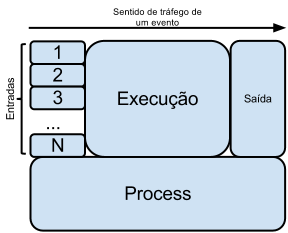
\includegraphics{basic_component.png}}
  \caption{rquitetura básica de um componente primitivo.}
\label{fig:basic_component}
\end{figure}

\begin{figure}
  \centerline{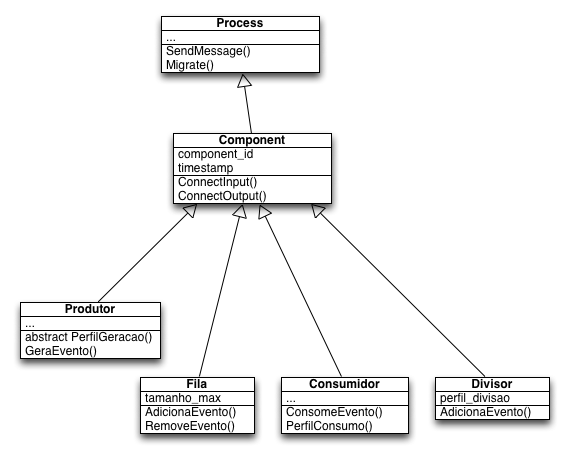
\includegraphics{uml_componentes.png}}
  \caption{Hierarquia dos componentes básicos.}
\label{fig:uml_components}
\end{figure}

Sobre este componente primitivo são construídos quatro componentes básicos, suficientes para demonstrar a implementação de alguns modelos para simulação. Estes componentes são: fila, gerador, consumidor e divisor.

Cada um desses componentes é construído sobre a arquitetura do componente primitivo descrito na seção~\ref{primitivo}. Por motivos naturais, nem todos os componentes implementos esse modelo em sua totalidade. Componentes como os geradores de eventos, por exemplo, não possuem canais de entrada de eventos, uma vez que a sua função é a de apenas gerar novos eventos com base em uma parametrização de suas características para que se comporte conforme o modelo que descreve suas ações. 

\subsection{O componente Fila}

A fila é o o ponente responsável por armazenar eventos, ordenando-os com base no seu \textit{timestamp}. Cada evento que chega à fila é alocado respeitando a ordem referente ao seu \textit{timestamp}, e cada vez que um elemento é retirado da fila, isto é feito retirando-se o primeiro elemento da fila, ou seja, o elemento com o menor \textit{timestamp}. 

A fila é um componente passivo, ou seja, ela não executa nenhum tipo de ação sobre os eventos nela existente. Por ser um componente passivo, é o componente gerador que deve executar a ação de inserir um novo evento na fila, e é um componente consumidor que deve executar a ação de retirar o evento de menor \textit{timestamp} da fila.

Uma das características mais importantes do componente fila é o seu tamanho. Uma fila pode ou não ter um tamanho definido, porém uma vez definido um tamanho para esta fila, quando este tamanho se excede, ou seja, quando a quantidade de eventos inseridos cresce em uma velocidade tão grande que o consumidor atrelado àquela fila não consegue consumi-los em tempo hábil podem ocorrer dois eventos, dependendo de como o usuário do framework descreveu em seu modelo. No caso mais simples o usuário determina que ao se exceder a quantidade de elementos em uma fila, uma excessão do tipo QueueOverflow() seja lançada, e a simulação se encerra.

Em um caso mais elaborado, ao se atingir o limite de uma fila esta pode apenas negar a inserção de novos elementos até que haja espaço suficiente. Neste caso, há uma propagação da condição de estacionamento da execução para os elementos atrelados à essa fila, causando um efeito que reflete em grande parte do sistema. 

\begin{figure}
  \centerline{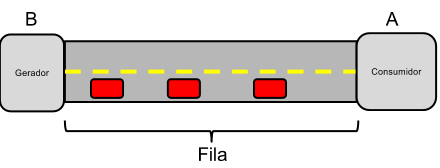
\includegraphics{cruzamento.png}}
  \caption{Modelagem de uma via urbana.}
\label{fig:cruzamento}
\end{figure}

Um exemplo típico que ilustra esse caso é a simulação de uma sequência de cruzamentos em uma via urbana, ilustrada na Figura~\ref{fig:cruzamento}. A quantidade de carros que cabem em um intervalo entre os dois cruzamentos A e B é finito, e se o cruzamento A não consome carros em uma velocidade maior ou igual à que eles chegam, há um crescimento na quantidade de carros entre os dois cruzamentos, o que pode levar à paralização temporária da simulação, até que o consumidor A consuma eventos, liberando espaço na fila.

\subsection{O componente Gerador}

Assim como ilustrado na Figura~\ref{fig:cruzamento}, um exemplo de gerador de eventos é uma extremidade de uma via de trânsito, que gera eventos (no exemplo citado, carros) em uma determinada taxa de tempo, com uma determinada frequência.

Um dos comportamentos parametrizáveis do componente gerador é a função que modela a taxa de criação de novos eventos ao longo do tempo. Um sistema que se deseja

\subsection{O componente Consumidor}
\subsection{O componente Divisor}

\section{O \textit{kernel} do \textit{framework}}


\section{Protocolos de sincronização}


\section{Algoritmos de balanceamento de carga}
